\section{Methodology and Implementation}
\label{sec:method}



\begin{figure*}[!t]
\centering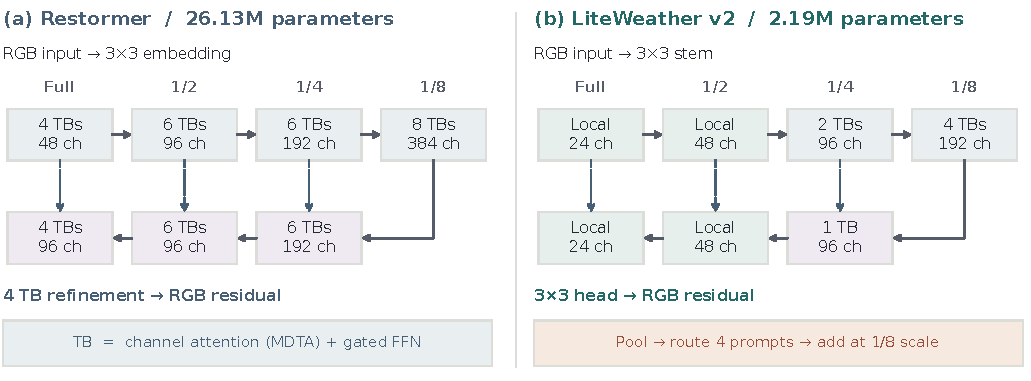
\includegraphics[width=\textwidth]{figures/restorer_architectures.pdf}
\caption{Architectures evaluated on the paired benchmark. Restormer uses transformer blocks (TBs) at all four scales. LiteWeather v2 uses local residual blocks at full and half resolution and attention at quarter and eighth resolution. Its soft prompt mixture is added before the eighth-scale transformer blocks. Arrows between scales represent down/up-sampling. Dashed arrows show encoder-to-decoder concatenation. Each network predicts a residual added to the degraded RGB image.}
\label{fig:architecture}
\end{figure*}

\paragraph{Shared training schedule.}
All six recipes use seed 42, 60 epochs, global batch four, and 4,096 paired draws per epoch with random $256\times256$ crops and flips. Background-aware sampling with replacement uses rain/fog/snow/smoke probabilities of 0.30/0.30/0.30/0.10. The non-GAN runs use L1 and AdamW, a $10^{-4}$ learning rate decayed to $10^{-6}$, $10^{-4}$ weight decay, and gradient clipping at 1.0. Attention Pix2Pix uses Adam, a patch discriminator, and adversarial loss plus $100$-weighted L1. BF16 training runs use an A100-SXM4-40GB. The best native-resolution validation macro PSNR selects the checkpoint.

\paragraph{Initialization and model identity.}
Attention Pix2Pix and LiteWeather v2 start from initialization. Restormer and RAMiT start from verified deraining weights, TransWeather from All-Weather weights, and PromptIR from its all-in-one weights. The published models use pinned sources and strict checkpoint loading. These recipes differ in prior data exposure.

\paragraph{Restormer.}
The epoch-51 model (26.13M parameters) connects the follow-up,
detection and export studies. Its encoder widths are $[48,96,192,384]$,
block counts $[4,6,6,8]$, and head counts $[1,2,4,8]$, with four refinement
blocks after decoding (Fig.~\ref{fig:architecture}a). All layers are fine-tuned;
selected weights are then frozen for evaluation and export~\cite{Zamir_2022_CVPR}.

\paragraph{Compact comparator.}
LiteWeather v2 (2.19M parameters) uses local residual blocks at full and
half resolution, two attention blocks at quarter scale and four at eighth
scale, with four and eight heads respectively (Fig.~\ref{fig:architecture}b).
A learned prompt mixture conditions its latent features without weather labels.

\subsection{Attention and residual reconstruction}
The implemented Restormer forms query, key and value tensors with a
$1\times1$ convolution followed by a depthwise $3\times3$ convolution.
Within each head, $Q$ and $K$ are normalized along the spatial dimension.
With $c_h$ channels per head and $n$ spatial positions, they have shape
$c_h\times n$. The implemented attention is
\begin{equation}
 A=\softmax(\tau\,\bar Q\bar K^\top),\qquad
 Z=W_o(AV),
\end{equation}
where $A$ has shape $c_h\times c_h$ and $\tau$ is a learned temperature.
Layer normalization and residual connections surround attention and the
feed-forward sublayer. That sublayer splits depthwise-filtered projected
features into $U$ and $V$, gates them as $\operatorname{GELU}(U)\odot V$,
and projects back to the block width. The decoder uses upsampling and skip
concatenation, followed by refinement and an RGB residual added to the input.
These are the existing Restormer mechanisms.

LiteWeather v2 conditions its latent representation $F$ using four learned
prompt vectors $p_j$:
\begin{equation}
 \alpha=\softmax(W_r\GAP(F)+b_r),\qquad
 F'=F+\sum_{j=1}^{4}\alpha_jp_j.
\end{equation}
The router receives image features rather than ground-truth weather labels.
The evaluated checkpoint uses widths $[24,48,96,192]$. The preserved earlier
convolution-only LiteWeather module is a different model.

\subsection{Model loading and identity}
Pinned upstream implementations use strict state loading: shape or key
mismatches are rejected. The selected Restormer inference package retains
26,126,644 parameters in 104,701,712 bytes. Continuation, downstream and export
studies use this same checkpoint; the historical rain-only checkpoint is
separate. The shared comparison evaluates complete training recipes, including
the differing initialization sources and objectives described above.

\subsection{Controlled adapter design}
The experimental context/detail adapter is inserted after the latent and
third-level decoder stages while preserving backbone parameter names.
It normalizes and reduces features to width 64. A $5\times5$ average filter
forms a low-frequency estimate, and subtracting it forms a local high-pass
component. A sigmoid gate receives mean absolute low/high feature magnitudes.
The spatial branch pools to an $8\times8$ token grid and applies four-head
spatial attention; the detail branch filters the high-pass component with
a depthwise $5\times5$ kernel and GELU.

Zero-initialized output projections preserve the starting backbone.
Spatial-attention logits and softmax remain FP32 under mixed precision.
This enables matched spatial-only, detail-only and combined arms. Average
filtering is an implementation choice, not a physical separation of weather
and scene content (Section~\ref{sec:jointresults}).
